\section{Trust in the proof and VST}
\label{sec5-vst}

Any formal system relies on a trusted base. In this section we describe our
chain of trust bringing up to light some tripping points a user may encounter
when using VST.

\subsection{The Trusted Base}

Our proof relies on a trusted base , i.e. a foundation of specifications
and implementations that must stay correct with respect to their specifications.
One should not be able to prove a false statement in that system e.g. by proving
an inconsistency.

In our case we rely on:
\begin{itemize}
  \item \textbf{Calculus of Inductive Construction}. The intuitionistic logic
  used by Coq must be consistent in order to trust the proofs. As an axiom,
  we assumed that the functional extensionality, which is also consistent with that logic.
  $$\forall x, f(x) = g(x) ) \implies f = g$$
\begin{lstlisting}[language=Coq]
Lemma f_ext: forall (A B:Types),
  forall (f g: A -> B),
  (forall x, f(x) = g(x)) -> f = g.
\end{lstlisting}

  \item \textbf{Verifiable Software Toolchain}. This framework developped at
  Princeton allows a user to prove that a \texttt{CLight} code matches pure Coq
  specification. However one must trust that the framework properly captures and
  map the CLight behavior to the basic pure Coq functions. At the begining of
  the project we found inconsistency and reported them to the authors.

  \item \textbf{CompCert}. The formally proven compiler. We trust that the Clight
  model captures correctly the C standard. (VERIFY THIS, WHICH STANDARD ?).
  Our proof also assumes that the TweetNaCl code will behave as expected if
  compiled under CompCert. We do not provide garantees for other C compilers
  such as Clang or GCC.

  \item \textbf{\texttt{clightgen}}. The tool making the translation from \textbf{C} to
  \textbf{Clight}. It is the first step of the compilation.
  VST does not support the direct verification of \texttt{o[i] = a[i] + b[i]}.
  This required us to rewrite the lines into:
\begin{lstlisting}[language=C]
aux1 = a[i];
aux2 = b[i];
o[i] = aux1 + aux2;
\end{lstlisting}
  The trust of the proof relied on the trust of a correct translation from the
  initial version of \textit{TweetNaCl} to \textit{TweetNaclVerificable}.

  While this problem is still present, the Compcert developpers provided us with
  the \texttt{-normalize} option for \texttt{clightgen} which takes care of
  generating auxiliary variables in order to automatically derive these steps.
  The changes required for a C-code to make it Verifiable are now minimal.

  \item Last but not the least, we must trust: the \textbf{Coq kernel} and its
  associated libraries; the \textbf{Ocaml compiler} on which we compiled Coq;
  the \textbf{Ocaml Runtime} and the \textbf{CPU}. Those are common to all proofs
  done with this architecture \cite{2015-Appel,coq-faq}.
\end{itemize}

\subsection{Using the Verifiable Software Toolchain}

The Verifiable Software Toolchain uses a strongest postcondition strategy.
The user must first write a formal specification of the function he wants to verify in Coq.
This should be as close as possible to the C implementation behavior.
This will simplify the proof and help with stepping throught the CLight version of the software.
With the range of inputes defined, VST steps mechanically through each instruction
and ask the user to verify auxiliary goals such as array bound access, or absence of overflows/underflows.
We call this specification a low level specification. A user will then have an easier
time to prove that his low level specification matches a simpler higher level one.

In order to further speed-up the verification process, it has to be know that to
prove \VSTe{crypto_scalarmult}, a user only need the specification of e.g. \VSTe{M}.
This provide with multiple advantages: the verification by the Coq kernel can be done
in parallel and multiple users can work on proving different functions at the same time.
For the sake of completeness we proved all intermediate functions.

Memory aliasing is the next point a user should pay attention to. The way VST
deals with the separation logic is similar to a consumer producer problem.
A simple specification of \texttt{M(o,a,b)} will assume three distinct memory share.
When called with three memory share (\texttt{o, a, b}), the three of them will be consumed.
However assuming this naive specification when \texttt{M(o,a,a)} is called (squaring),
the first two memory shares (\texttt{o, a}) are consumed and VST will expect a third
memory share where the last \texttt{a} is pointing at which does not \textit{exist} anymore.

Examples of such cases are summarized in Fig \ref{tk:MemSame}.
\begin{figure}[h]
  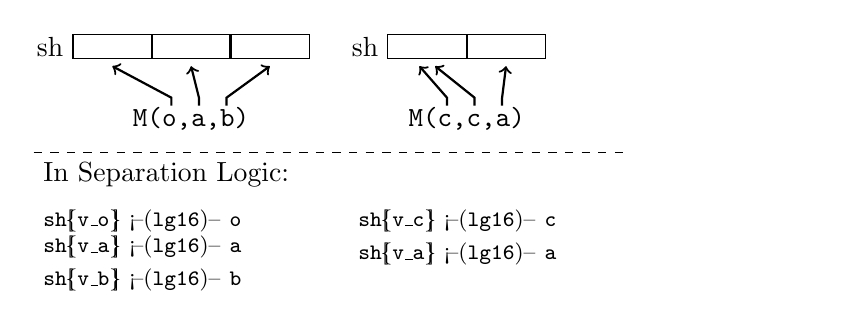
\begin{tikzpicture}
\def\-{\raisebox{.75pt}{-}}

\draw (0,0) rectangle (3,0.3);
\draw[thick] (1,0) -- (1,0.3);
\draw[thick] (2,0) -- (2,0.3);
\node [anchor=east] (shn) at (0,0.15) {sh};
\node [anchor=north] (Moab) at (1.5,-0.5) {\texttt{M(o,a,b)}};
\draw[thick, -> ] (1.25, -0.6) -- (1.25, -0.5) -- (0.5,-0.1);
\draw[thick, -> ] (1.6, -0.6) -- (1.6, -0.5) -- (1.5,-0.1);
\draw[thick, -> ] (1.95, -0.6) -- (1.95, -0.5) -- (2.5,-0.1);

\node [anchor=north west, text width=6cm, align=left] (Sepoab) at (-0.5,-1.8)
  {\footnotesize{$\mathtt{sh [\!\!\{ v\_o \}\!\!]\ \textrm{<\!--(}lg16\textrm{)--}\ o}$\\
  $\mathtt{sh [\!\!\{ v\_a \}\!\!]\ \textrm{<\!--(}lg16\textrm{)--}\ a}$\\
  $\mathtt{sh [\!\!\{ v\_b \}\!\!]\ \textrm{<\!--(}lg16\textrm{)--}\ b}$}};


\begin{scope}[yshift=0 cm,xshift=4 cm]
  \draw (0,0) rectangle (2,0.3);
  \draw[thick] (1,0) -- (1,0.3);
  % \draw[thick] (2,0) -- (2,0.3);
  \node [anchor=east] (shm) at (0,0.15) {sh};
  \node [anchor=north] (Mcaa) at (1,-0.5) {\texttt{M(c,c,a)}};
  \draw[thick, -> ] (0.75, -0.6) -- (0.75, -0.5) -- (0.4,-0.1);
  \draw[thick, -> ] (1.1, -0.6) -- (1.1, -0.5) -- (0.6,-0.1);
  \draw[thick, -> ] (1.45, -0.6) -- (1.45, -0.5) -- (1.5,-0.1);

  \node [anchor=north west, text width=6cm, align=left] (Sepoab) at (-0.5,-1.8)
    {\footnotesize{$\mathtt{sh [\!\!\{ v\_c \}\!\!]\ \textrm{<\!--(}lg16\textrm{)--}\ c}$\\
    $\mathtt{sh [\!\!\{ v\_a \}\!\!]\ \textrm{<\!--(}lg16\textrm{)--}\ a}$}};

\end{scope}

\draw[dashed] (-0.5,-1.2) -- +(7.5,0);
\node [anchor=north west] (sep) at (-0.5,-1.2) {In Separation Logic:};

\end{tikzpicture}

  \caption{Aliasing and Separation Logic}
  \label{tk:MemSame}
\end{figure}

This forces the user to either define multiple specifications for a single function
or specify in his specification which aliasing version is being used.
For our specifications of functions with 3 arguments, named here after \texttt{o, a, b},
we define an additional parameter $k$ with values in
$\{0,1,2,3\}$:
\begin{itemize}
  \item if $k=0$ then \texttt{o} and \texttt{a} are aliased.
  \item if $k=1$ then \texttt{o} and \texttt{b} are aliased.
  \item if $k=2$ then \texttt{a} and \texttt{b} are aliased.
  \item else there is no aliasing.
\end{itemize}
This solution allows us to make cases analysis over possible aliasing.

\subsection{Verifiying \texttt{for} loops}

Final state of \texttt{for} loops are usually computed by simple recursive functions.
However we must define invariants which are true for each iterations.

Assume we want to prove a decreasing loop where indexes go from 3 to 0.
Define a function $g : \N \rightarrow State  \rightarrow State $ which takes as input an integer for the index and a state and return a state.
It simulate the body of the \texttt{for} loop.
Assume it's recursive call: $f : \N \rightarrow State \rightarrow State $ which iteratively apply $g$ with decreasing index:
\begin{equation*}
  f ( i , s ) =
  \begin{cases}
  s & \text{if } s = 0 \\
  f( i - 1 , g ( i - 1  , s )) & \text{otherwise}
  \end{cases}
\end{equation*}
Then we have :
\begin{align*}
  f(4,s) &= g(0,g(1,g(2,g(3,s))))
  % \\
  % f(3,s) &= g(0,g(1,g(2,s)))
\end{align*}
To prove the correctness of $f(4,s)$, we need to prove that intermediate steps
$g(3,s)$; $g(2,g(3,s))$; $g(1,g(2,g(3,s)))$; $g(0,g(1,g(2,g(3,s))))$ are correct.
Due to the computation order of recursive function, our loop invariant for $i\in\{0;1;2;3;4\}$ cannot use $f(i)$.
To solve this, we define an auxiliary function with an accumulator such that given $i\in\{0;1;2;3;4\}$, it will compute the first $i$ steps of the loop.
We then prove for the complete number of steps, the function with the accumulator and without returns the same result.

We formalized this result in a generic way as follows:
\begin{Coq}
Variable T : Type.
Variable g : nat -> T -> T.

Fixpoint rec_fn (n:nat) (s:T) :=
  match n with
  | 0 => s
  | S n => rec_fn n (g n s)
  end.

Fixpoint rec_fn_rev_acc (n:nat) (m:nat) (s:T) :=
  match n with
  | 0 => s
  | S n => g (m - n - 1) (rec_fn_rev_acc n m s)
  end.

Definition rec_fn_rev (n:nat) (s:T) :=
  rec_fn_rev_acc n n s.

Lemma Tail_Head_equiv :
  forall (n:nat) (s:T),
  rec_fn n s = rec_fn_rev n s.
\end{Coq}
Using this formalization, we prove that the 255 steps of the montgomery ladder in C provide the same computations are the one defined in Algorithm \ref{montgomery-double-add}.

\subsection{Time and Space Complexity}

Our work can be split into multiple parts. Bellow we provide an approximation of
the number of lines of codes and thus an idea of the size of the proofs required to
complete this work.
\begin{itemize}
  \item The proof that the Montgomery ladder over a generic field $\K$ respects
  the elliptic curve theory and then it's specialization for $\F{p^2}$.
  This represent 4218 lines of code for 0.75 man-year.
  \item The multiple level definitions of the ladder and operations over lists,
  their proof of correctness and soundness and additionally that the match with
  the generic Montgomery ladder. This count for 22967 lines of code for about 1.5 man-year.
  \item The proof that our specification matches the Clight translation with VST.
  This count for 6934 lines of code for about 0.75 man-year.
\end{itemize}
While the proof with VST took slightly less time, having to provide proof that every
intermediate computations slows down the process significantly. However it is
necessary in order to garantee our the absences of overflows and underflows.
